\section{Results}

The results section should be based on the following graphs.

\begin{figure}
	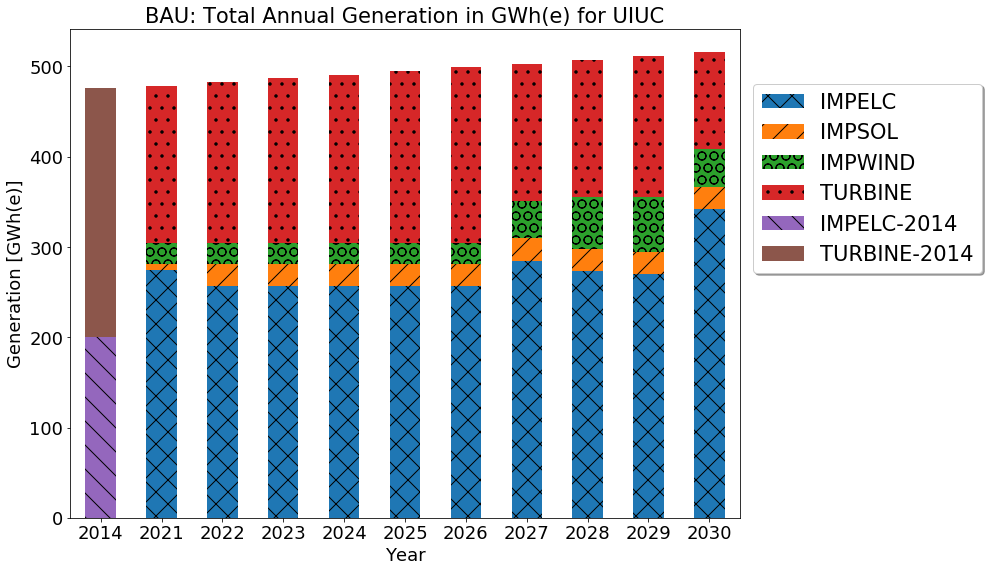
\includegraphics[width=\columnwidth]{bau_generation_w2014.png}
	\caption{Business as usual electricity generation.}
	\label{fig:bau_generation}
\end{figure}
\begin{figure}
	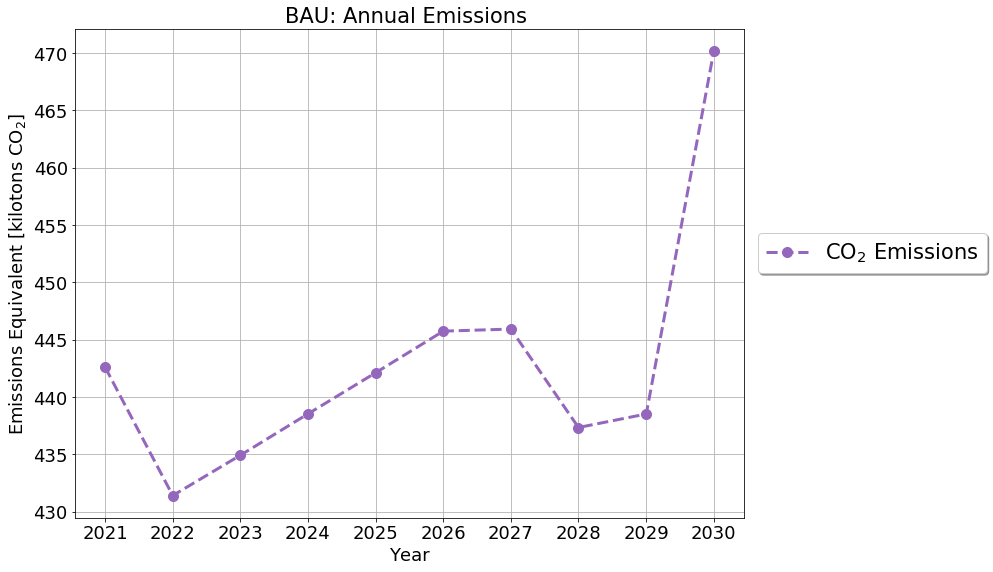
\includegraphics[width=\columnwidth]{bau_emissions.png}
	\caption{Business as usual carbon emissions.}
	\label{fig:bau_emissions}
\end{figure}
\begin{figure}
	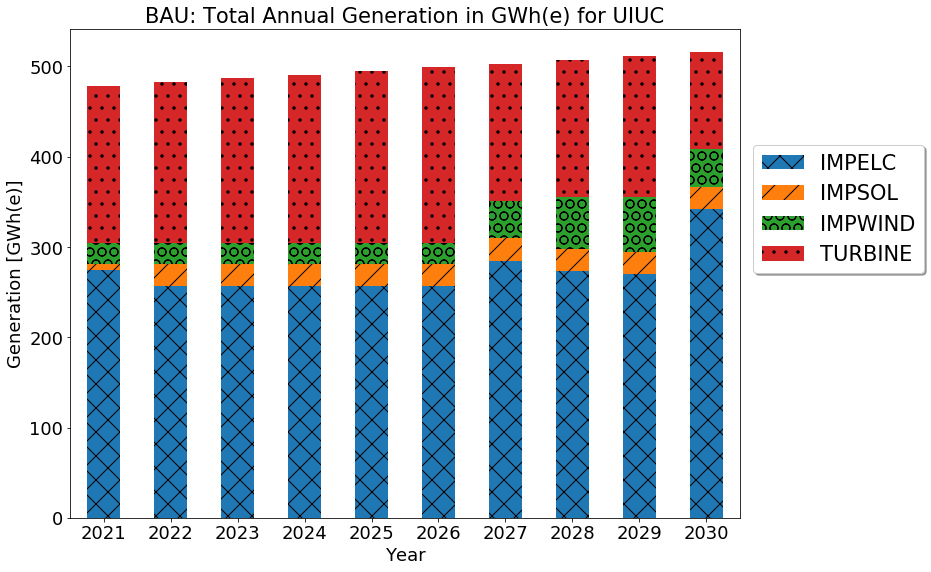
\includegraphics[width=\columnwidth]{bau_generation.png}
	\caption{Business as usual electricity generation.}
	\label{fig:}
\end{figure}
\begin{figure}
	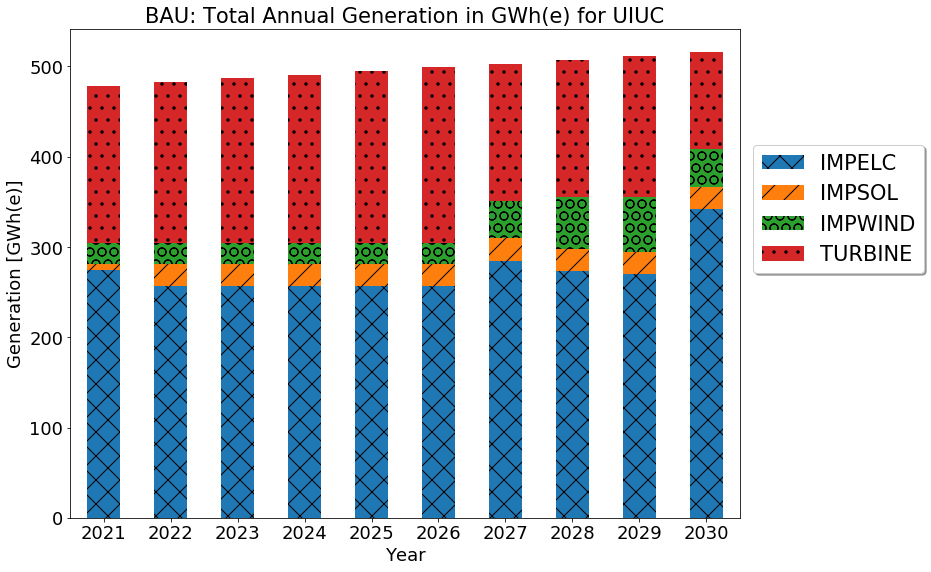
\includegraphics[width=\columnwidth]{bau_generation.png}
	\caption{Business as usual electricity generation.}
	\label{fig:}
\end{figure}
\begin{figure}
	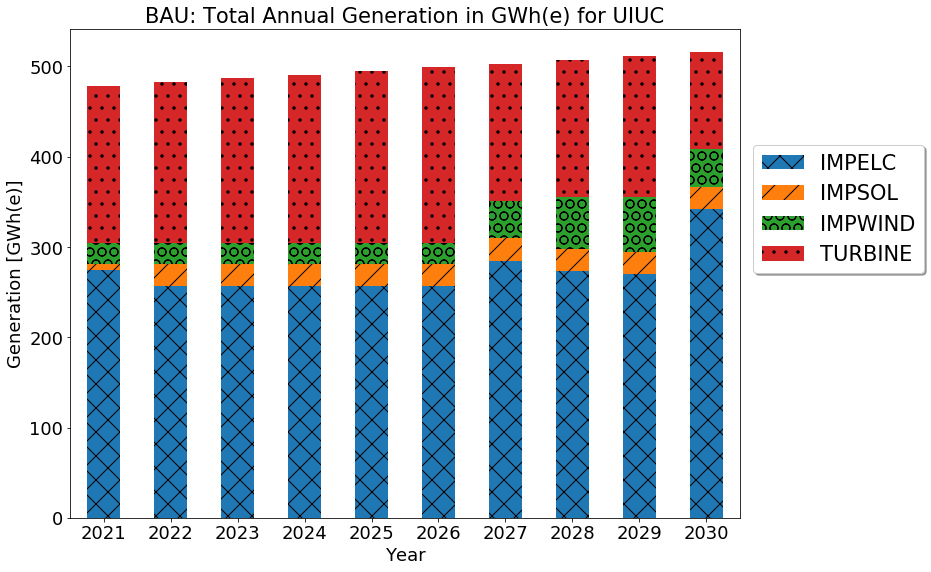
\includegraphics[width=\columnwidth]{bau_generation.png}
	\caption{Business as usual electricity generation.}
	\label{fig:}
\end{figure}
\begin{figure}
	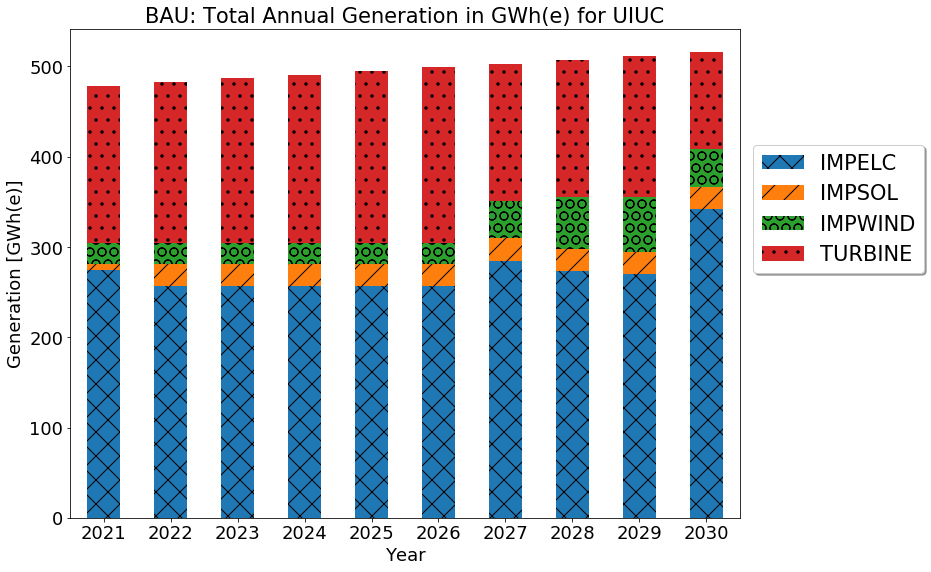
\includegraphics[width=\columnwidth]{bau_generation.png}
	\caption{Business as usual electricity generation.}
	\label{fig:}
\end{figure}
\begin{figure}
	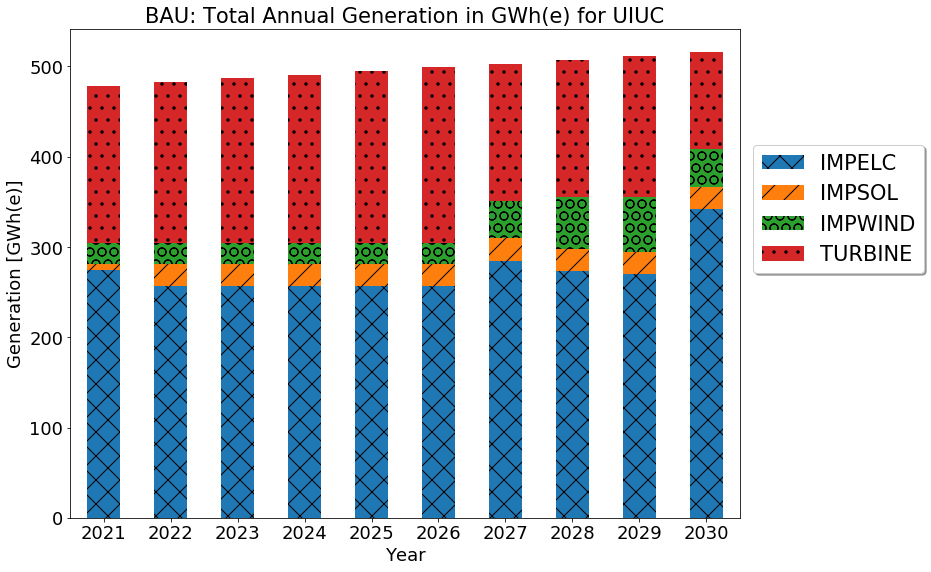
\includegraphics[width=\columnwidth]{bau_generation.png}
	\caption{Business as usual electricity generation.}
	\label{fig:}
\end{figure}
\begin{figure}
	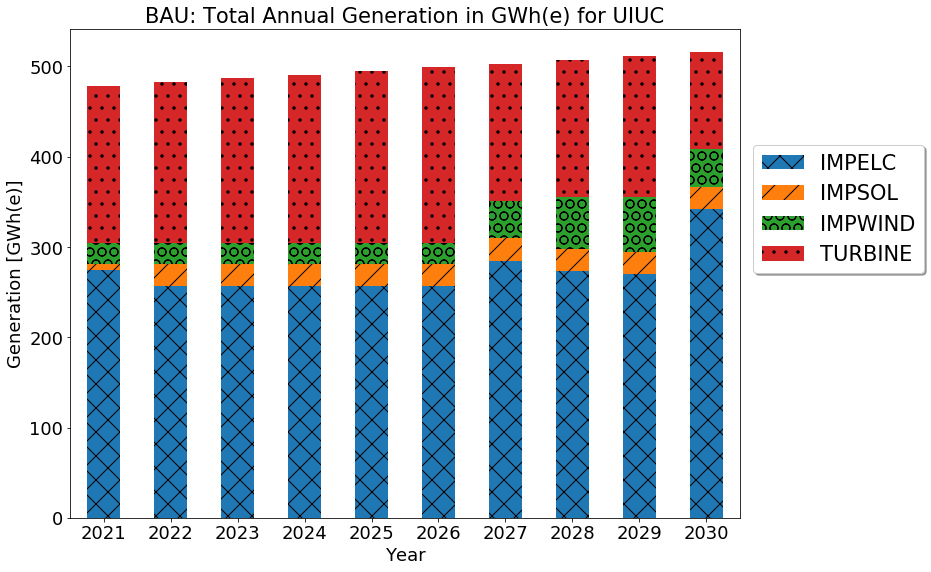
\includegraphics[width=\columnwidth]{bau_generation.png}
	\caption{Business as usual electricity generation.}
	\label{fig:}
\end{figure}
\begin{figure}
	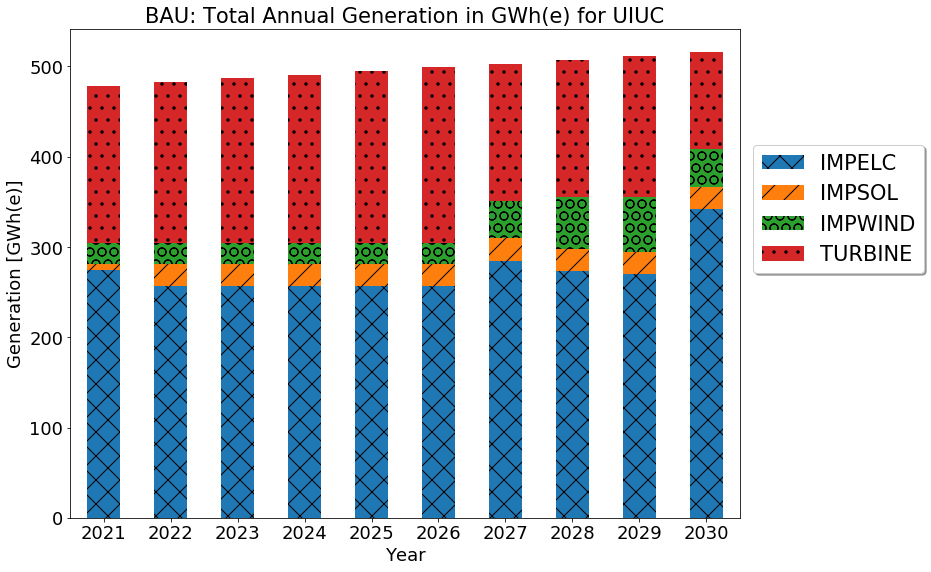
\includegraphics[width=\columnwidth]{bau_generation.png}
	\caption{Business as usual electricity generation.}
	\label{fig:}
\end{figure}
\begin{figure}
	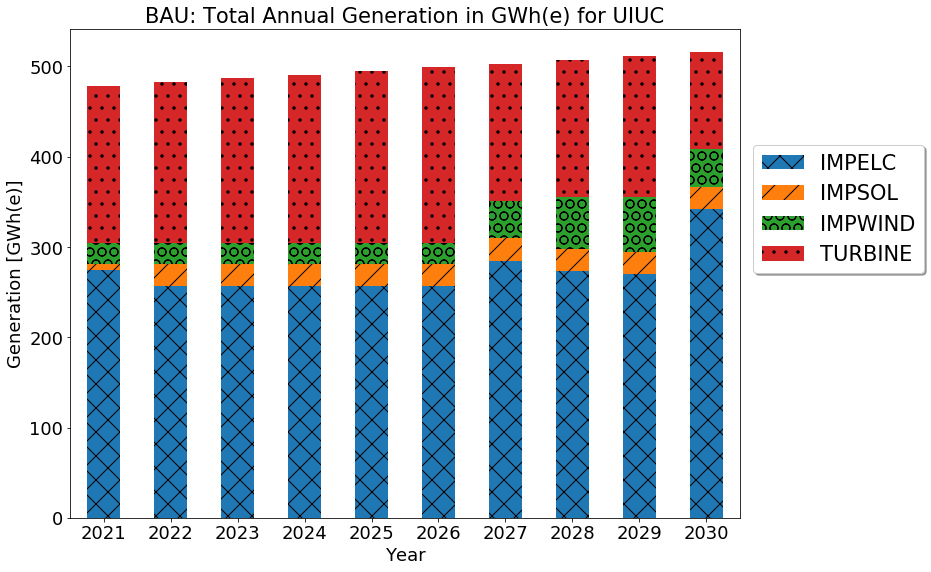
\includegraphics[width=\columnwidth]{bau_generation.png}
	\caption{Business as usual electricity generation.}
	\label{fig:}
\end{figure}
\begin{figure}
	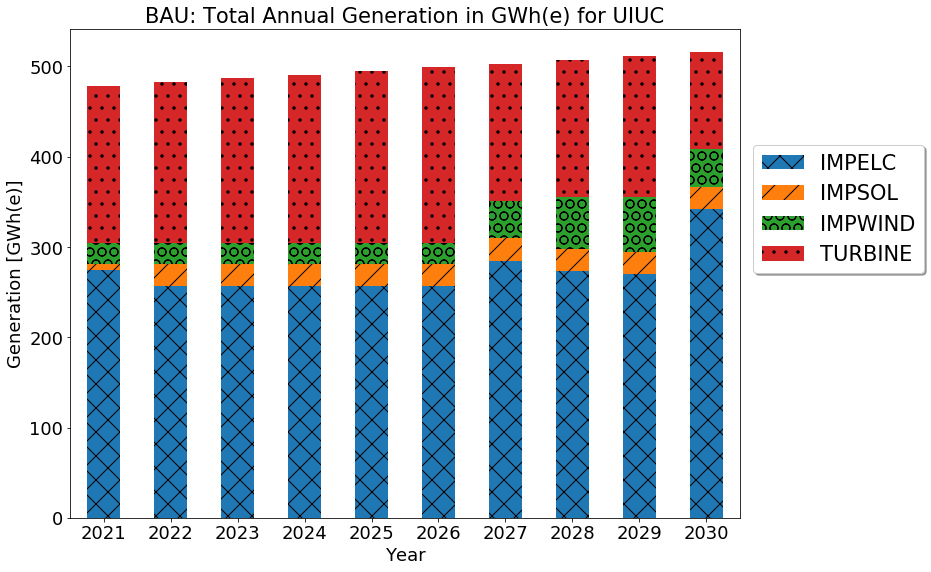
\includegraphics[width=\columnwidth]{bau_generation.png}
	\caption{Business as usual electricity generation.}
	\label{fig:}
\end{figure}
